\subsection{UC1 - Registrazione utente base}\label{usecase:1}
\begin{figure}[H]
  \centering
  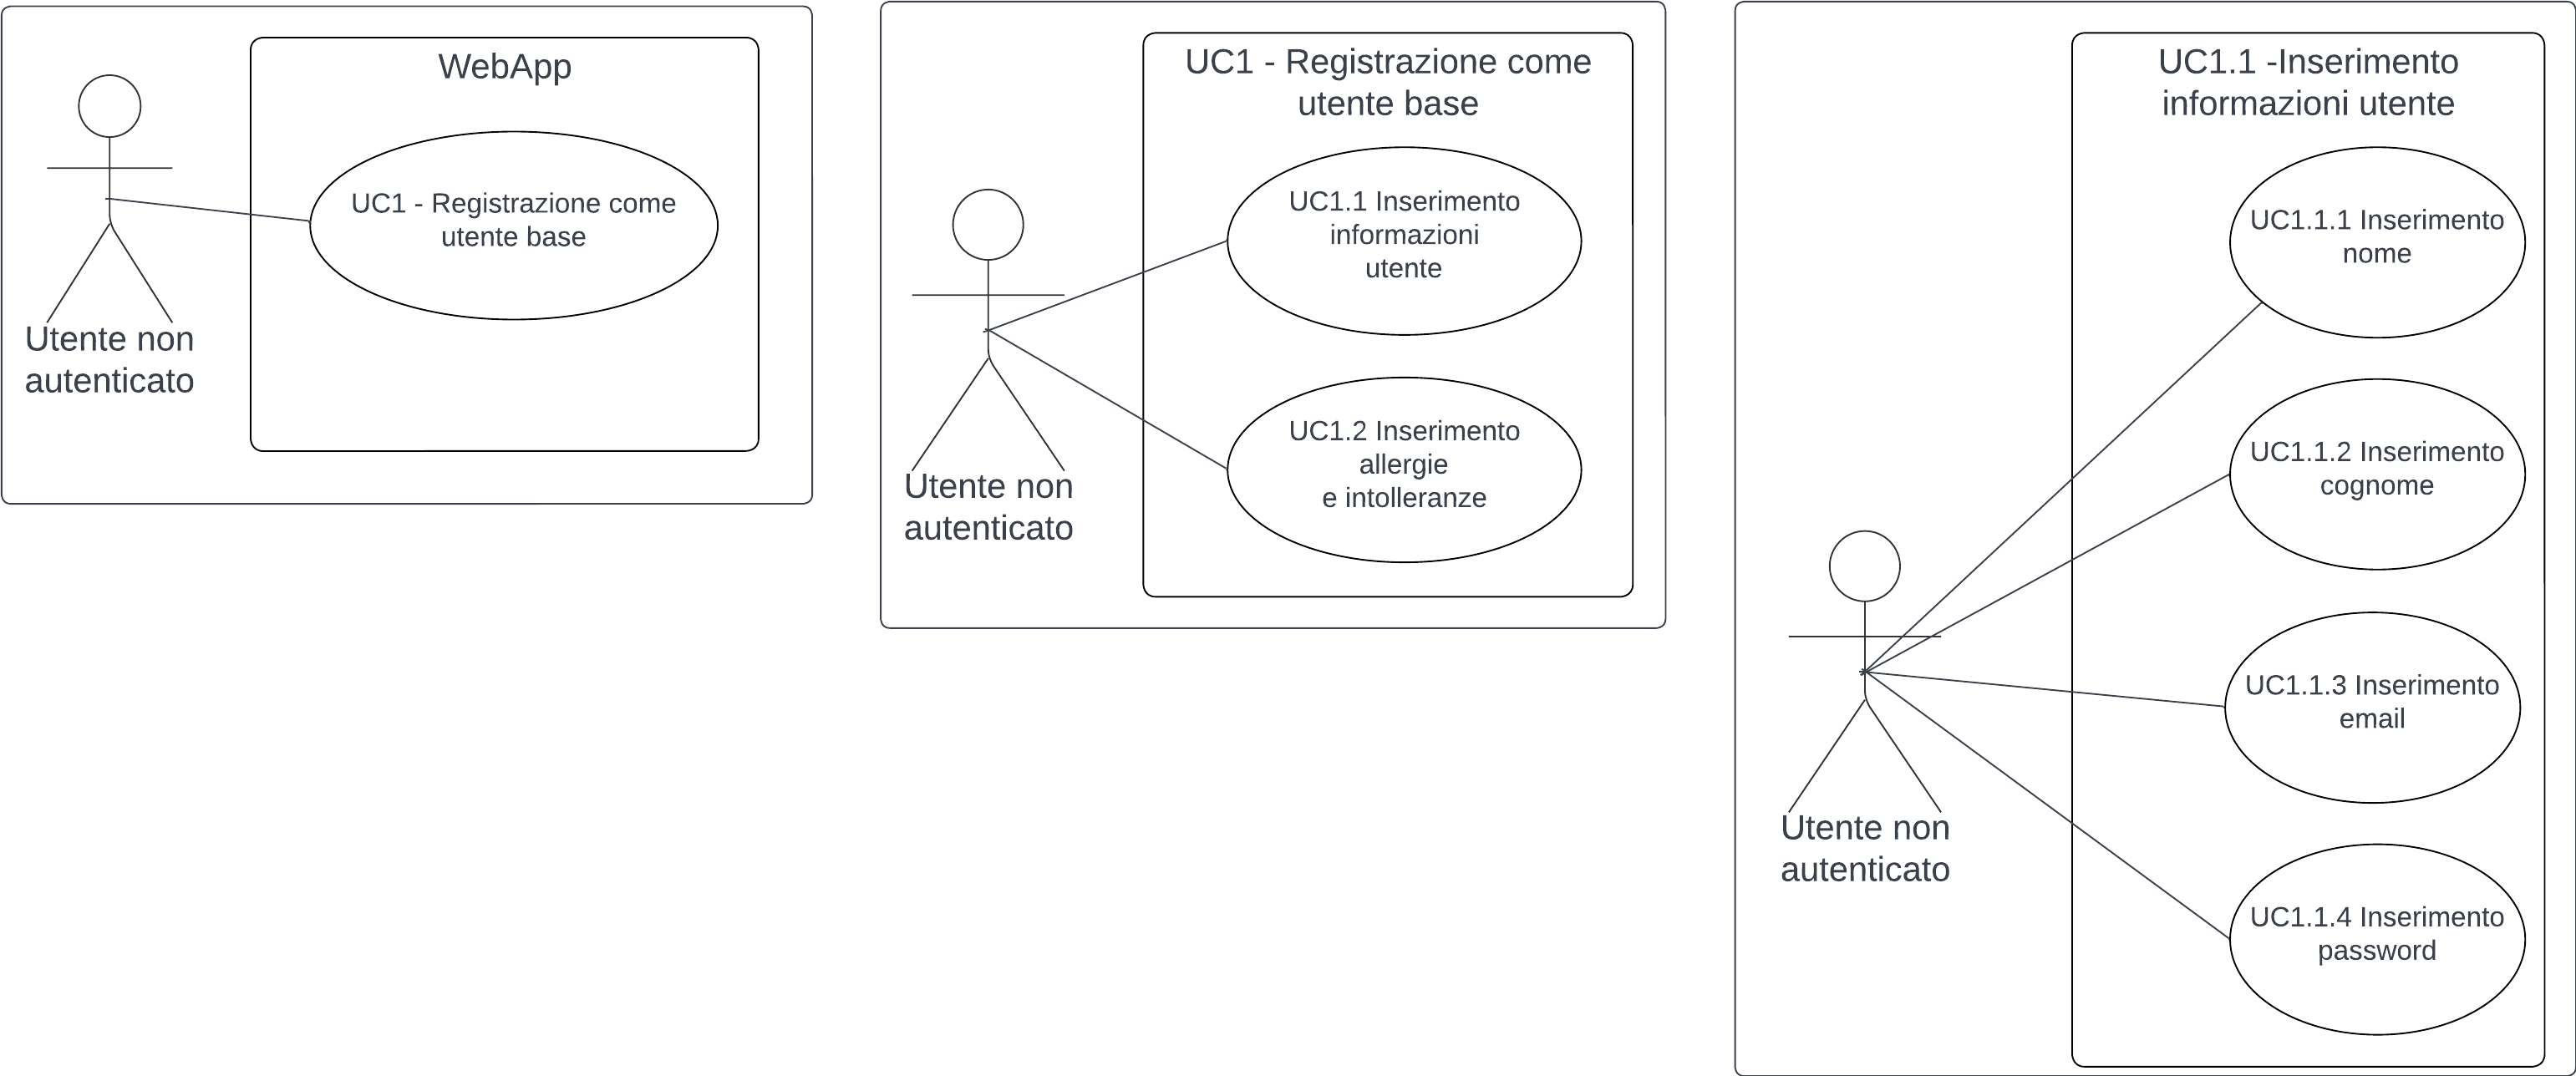
\includegraphics[width=0.9\linewidth]{ucd/UCD1_finale.png}
\caption{Registrazione come utente base}
\end{figure}
\textbf{Attori principali}: 
\begin{itemize}
    \item Utente non autenticato.
\end{itemize}
\textbf{Precondizioni}:
\begin{itemize}
    \item L'utente è connesso al $\textit{Sistema}_G$.
\end{itemize}
\textbf{Postcondizioni}: 
\begin{itemize}
    \item L'utente si è registrato ed è riconosciuto dal $\textit{Sistema}_G$ come utente base.
\end{itemize}
\textbf{Scenario principale}:
\begin{enumerate}
    \item L'utente inserisce le sue credenziali (\nameref{usecase:1_1}).
    \item L'utente inserisce allergie e intolleranze se presenti (\nameref{usecase:1_2});
    \item L'utente conferma di volersi registrare con le informazioni fornite.
\end{enumerate}
\textbf{Scenari alternativi}:
\begin{enumerate}
    \item Inserimento informazioni utente errate
    \item Viene visualizzato un errore;
    \item L'utente decide se annullare o riprovare
\end{enumerate}

\begin{comment}
\textbf{Scenari alternativi}:
\begin{itemize}
    \item Inserimento informazioni utente errate: 
    \begin{enumerate}
        \item Campo nome:
        \begin{enumerate}
            \item L'utente lascia il nome vuoto;
            \item L'utente usa solo spazi (" ");
            \item L'utente usa caratteri speciali;
            \item L'utente usa caratteri numerici;
        \end{enumerate}
        \item Campo cognome:
        \begin{enumerate}
            \item L'utente lascia il cognome vuoto;
            \item L'utente usa solo spazi (" ");
            \item L'utente usa caratteri speciali;
            \item L'utente usa caratteri numerici;
        \end{enumerate}
        \item Campo email:
        \begin{enumerate}
            \item L'utente lascia il campo email vuoto;
            \item L'utente non inserisce una email nel formato: xxxxx@yyy.zz;
            \item L'utente inserisce una email già registrata;
        \end{enumerate}
        \item Campo password:
        \begin{enumerate}
            \item L'utente lascia il campo password vuoto;
            \item L'utente inserisce una password troppo corta (minore di 6 caratteri);
            \item L'utente inserisce una password troppo lunga (maggiore di 24 caratteri);
            \item L'utente inserisce una password senza caratteri minuscoli;
            \item L'utente inserisce una password senza caratteri maiuscoli;
            \item L'utente inserisce una password senza caratteri numerici;
            \item L'utente inserisce una password senza caratteri speciali;
        \end{enumerate}
    \end{enumerate}
    \item Viene visualizzato un errore;
    \item L'utente decide se annullare o riprovare.
\end{itemize}

\end{comment}

\begin{comment}    
    1.1.  L'utente lascia il campo nome vuoto
    
    1.2.  L'utente lascia il campo cognome vuoto
    
    1.3a.  L'utente lascia il campo email vuoto
    
    1.3b.  L'utente non inserisce una email nel formato: xxxxx@yyy.zz
    
    1.3c.  L'utente inserisce una email già registrata
    
    1.4a.  L'utente lascia il campo password vuoto
    
    1.4b.  L'utente inserisce una password troppo corta (minore di 6 caratteri)
    
    1.4c.  L'utente inserisce una password troppo lunga (maggiore di 24 caratteri)
    
    1.4d.  L'utente inserisce una password senza caratteri minuscoli
    
    1.4e.  L'utente inserisce una password senza caratteri maiuscoli
    
    1.4f.  L'utente inserisce una password senza caratteri numerici
    
    1.4g.  L'utente inserisce una password senza caratteri speciali

    % 1.5. L'utente lascia il campo allergie e intolleranze vuoto
    
    2.  Viene visualizzato un errore esplicativo
    
    3.  Viene data la possibilità di rifare la registrazione come utente base
    \item L'utente decide di annullare l'operazione di registrazione
\end{comment}
\begin{comment}
\subsubsection{UC1 - Registrazione come utente base}\label{usecase:1}
\textbf{Attori}: 
\begin{itemize}
    \item Utente non autenticato
\end{itemize}
\textbf{Precondizioni}:
\begin{itemize}
    \item L'utente non è ancora autenticato
\end{itemize}
\textbf{Postcondizioni}: 
\begin{itemize}
    \item L'utente si è registrato ed è riconosciuto come utente base 
\end{itemize}
\textbf{Trigger}:
\begin{itemize}
    \item L'utente sceglie di registrarsi come utente base
\end{itemize}
\textbf{Scenario principale}:
\begin{enumerate}
    \item L'utente inserisce:
    \begin{enumerate}
        \item Nome
        \item Cognome
        \item Email valida %(\nameref{usecase:1_1})
        \item Passoword che rispetta i criteri indicati %(\nameref{usecase:1_2})
    \end{enumerate}
        \item l'utente \textbf{può} inserire eventuali allergie e intolleranze
\end{enumerate}
\textbf{Scenari secondari}:
\begin{enumerate}
    \item L'utente può decidere di interrompere l'operazione di registrazione in qualsiasi momento
    \item Nel caso in cui l'utente inserisca una mail non valida, oppure inserisca una password non valida, oppure lasci qualche campo obbligatorio vuoto:
    \begin{enumerate}
        \item L'utente non viene registrato presso il sistema
        \item Viene visualizzato un errore esplicativo
        \item Viene data la possibilità di rifare la registrazione come utente base
    \end{enumerate}
\end{enumerate}
\end{comment}